

\noindent
{\tt [{Foglio2-0}]} Il modulo del vettore $\vec{A}(3;4)$ è

{$A$}: 5\ \ 
{$B$}: 8\ \ 
{$C$}: 12\ \ 
{$D$}: 25\ \ 


\noindent
{\tt [{Foglio2-1}]} Il modulo del vettore $\vec{A}(2;2)$ è

{$A$}: boh\ \ 
{$B$}: non so\ \ 
{$C$}: chissà\ \ 
{$D$}: calcolalo da solo!\ \ 


\noindent
{\tt [{Foglio3-0}]} Di che colore era il cavallo bianco di Napoleone?

{$A$}: Bianco\ \ 
{$B$}: Verde\ \ 
{$C$}: Blu\ \ 
{$D$}: Marrone\ \ 
{$E$}: \ \ 


\noindent
{\tt [{Foglio4-0}]} Qual è la capitale d’Italia?

{$A$}: Roma\ \ 
{$B$}: Berlino\ \ 
{$C$}: Parigi\ \ 
{$D$}: Milano\ \ 
{$E$}: \ \ 


\noindent
{\tt [{Foglio6-0}]} Un gatto percorre 90,0~m verso sud e poi prosegue per altri 120~m verso ovest. Lo spostamento e la distanza percorsa sono rispettivamente

{$A$}: 150~m e 210~m\ \ 
{$B$}: 210~m e 150~m\ \ 
{$C$}: 210~m e 210~m\ \ 
{$D$}: 30~m e 210~m\ \ 
{$E$}: \ \ 


\noindent
{\tt [{Foglio7-0}]} Raddoppiando la distanza tra due cariche elettriche puntiformi, la forza elettrostatica diminuisce del

{$A$}: 75\%\ \ 
{$B$}: 50\%\ \ 
{$C$}: 25\%\ \ 
{$D$}: 90\%\ \ 
{$E$}: \ \ 


\noindent
{\tt [{Foglio8-0}]} Dato il vettore $\vec{d}$ in figura, determina il modulo e la componente $d_x$: \begin{figure}[h!]   \begin{center}     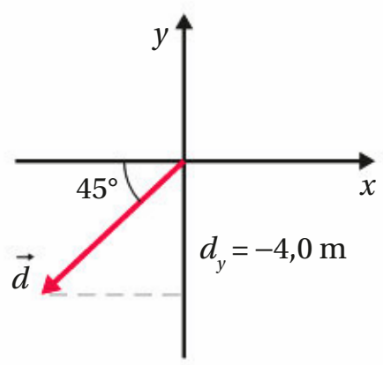
\includegraphics[scale=0.35]{vettored.png}   \end{center} \end{figure}

{$A$}: 5,7 m; -4,0 m\ \ 
{$B$}: -5,7 m; 4,0 m\ \ 
{$C$}: 5,7 m; 4,0 m\ \ 
{$D$}: -5,7 m; -4,0 m\ \ 
{$E$}: \ \ 


\noindent
{\tt [{Foglio9-0}]} I due vettori $\vec{a}$ e $\vec{b}$ hanno lo stesso modulo e la stessa direzione. Quale delle seguenti affermazioni è falsa?

{$A$}: Tutte le altre\ \ 
{$B$}: La loro somma è sicuramente nulla\ \ 
{$C$}: La loro somma non può mai essere zero\ \ 
{$D$}: I due vettori sono sicuramente uguali\ \ 
{$E$}: \ \ 


\noindent
{\tt [{Foglio10-0}]} Seguendo la mappa di un tesoro, un pirata cammina per 2,00~km verso nord-est, poi per 5,00~km verso est, quindi per 2,00~km verso sud-est e infine per 3,00~km verso ovest. Arrivato alla fine del percorso a che distanza si trova dalla posizione che occupava alla partenza?

{$A$}: 4,83 km\ \ 
{$B$}: 6,32 km\ \ 
{$C$}: 4,59 km\ \ 
{$D$}: 4,76 km\ \ 
{$E$}: \ \ 


\noindent
{\tt [{Foglio11-0}]} In quale anno il COVID ha fatto la sua comparsa?

{$A$}: 2019\ \ 
{$B$}: 2020\ \ 
{$C$}: 2001\ \ 
{$D$}: 1943\ \ 
{$E$}: \ \ 


\noindent
{\tt [{Foglio12-0}]} In che anno pare sia nato Gesù?

{$A$}: 0\ \ 
{$B$}: -80\ \ 
{$C$}: 2019\ \ 
{$D$}: 20\ \ 
{$E$}: \ \ 


\noindent
{\tt [{Foglio13-0}]} Se mischio blu e giallo che colore ottengo?

{$A$}: Verde\ \ 
{$B$}: Blallo\ \ 
{$C$}: Giallu\ \ 
{$D$}: Rosso\ \ 
{$E$}: \ \ 


\noindent
{\tt [{Foglio14-0}]} Come si chiama il satellite naturale della Terra?

{$A$}: Luna\ \ 
{$B$}: Sole\ \ 
{$C$}: ISS\ \ 
{$D$}: Marte\ \ 
{$E$}: \ \ 
